\subsection{Static Examples}
\label{sec:example:3dhex8-static}

PyLith features discussed in this example:
\begin{itemize}
\item Static solution
\item VTK output
\item Dirichlet displacement boundary conditions
\item Neumann traction boundary conditions
\item ZeroDispDB spatial database
\item SimpleDB spatial database
\item UniformDB spatial database
\item Static fault rupture
\item Specifying more than one material
\item Linearly elastic isotropic material
\end{itemize}

\subsubsection{Overview}

This set of examples describe the simplest class of problems for PyLith.
The problems are all purely elastic, and there is no time-dependence.
This set of elastostatic examples primarily demonstrates the application
of different types of boundary conditions in PyLith, as well as demonstrating
the use of a kinematic fault for a static problem. All of the examples
are contained in the directory \filename{examples/3d/hex8}, and the
corresponding \filename{cfg} files are \filename{step01.cfg}, \filename{step02.cfg},
and \filename{step03.cfg}. Run the examples as follows:
\begin{shell}
# Step01
$ pylith step01.cfg

# Step02
$ pylith step02.cfg

# Step03
$ pylith step03.cfg

\end{shell}
This will cause PyLith to read the default parameters in \filename{pylithapp.cfg},
and then override or augment them with the additional parameters in
the \filename{stepXX.cfg} file. Each \filename{cfg} file is extensively
documented to provide detailed information on the various parameters.


\subsubsection{Step01 - Pure Dirichlet Boundary Conditions}

The \filename{step01.cfg} file defines a problem with pure Dirichlet
(displacement) boundary conditions corresponding to compression in the
x-direction and shear in the y-direction. The bottom (minimum z)
boundary is held fixed in the z-direction. On the positive and
negative x-faces, compressional displacements of 1 m are applied in
the x-direction and shear displacements yielding a left-lateral sense
of shear are applied in the y-direction. In this example and in
subsequent examples we would like to output the displacement solution
over a subset of the domain corresponding to the ground surface.

\begin{cfg}[Excerpt from \filename{step01.cfg}]
<h>[pylithapp.timedependent.implicit]</h>
# Set the output to an array of 2 output managers.
# We will output the solution over the domain and the ground surface.
<f>output</f> = [domain,subdomain]

# Set subdomain component to OutputSolnSubset (boundary of the domain).
<f>output.subdomain</f> = pylith.meshio.OutputSolnSubset

# Give basename for VTK domain output of solution over ground surface.
<h>[pylithapp.problem.formulation.output.subdomain]</h>
# Name of nodeset for ground surface.
<p>label</p> = face_zpos
<p>writer.filename</p> = output/step01-groundsurf.vtk
\end{cfg}
For the boundary conditions, we must describe which degrees of freedom
are being constrained (\facility{bc\_dof}), we must provide a the label
associated with the CUBIT/Trelis nodeset associated with the BC, and we must
specify the type of spatial database is being used to describe the
boundary conditions. For the x-faces, we use a \object{SimpleDB} to
provide the displacements on the x-faces:
\begin{cfg}[Excerpt from \filename{step01.cfg}]
# Boundary condition on +x face
<h>[pylithapp.timedependent.bc.x_pos]</h>
<p>bc_dof</p> = [0, 1]
<p>label</p> = face_xpos
<f>db_initial</f> = spatialdata.spatialdb.SimpleDB
<p>db_initial.label</p> = Dirichlet BC on +x
<p>db_initial.iohandler.filename</p> = spatialdb/fixeddisp_axial_shear.spatialdb

# Boundary condition on -x face
<h>[pylithapp.timedependent.bc.x_neg]</h>
<p>bc_dof</p> = [0, 1]
<p>label</p> = face_xneg
<f>db_initial</f> = spatialdata.spatialdb.SimpleDB
<p>db_initial.label</p> = Dirichlet BC on -x
<p>db_initial.iohandler.filename</p> = spatialdb/fixeddisp_axial_shear.spatialdb
\end{cfg}
For a \object{SimpleDB}, we must provide a filename. The default spatial
database for \facility{db\_initial} is \object{ZeroDispBC}, which automatically
applies zero displacements to all vertices in the nodeset, and no
filename is required (or needed).
\begin{cfg}[Excerpt from \filename{step01.cfg}]
# Boundary condition on -z face
<h>[pylithapp.timedependent.bc.z_neg]</h>
<p>bc_dof</p> = [2]
<p>label</p> = face_zneg
<p>db_initial.label</p> = Dirichlet BC on -z
\end{cfg}
When we have run the simulation, the output VTK files will be contained
in \filename{examples/3d/hex8/output} (all with a prefix of \filename{step01}).
Results using ParaView are shown in Figure \vref{fig:example:3dhex8:step01:displacement}.

\begin{figure}
  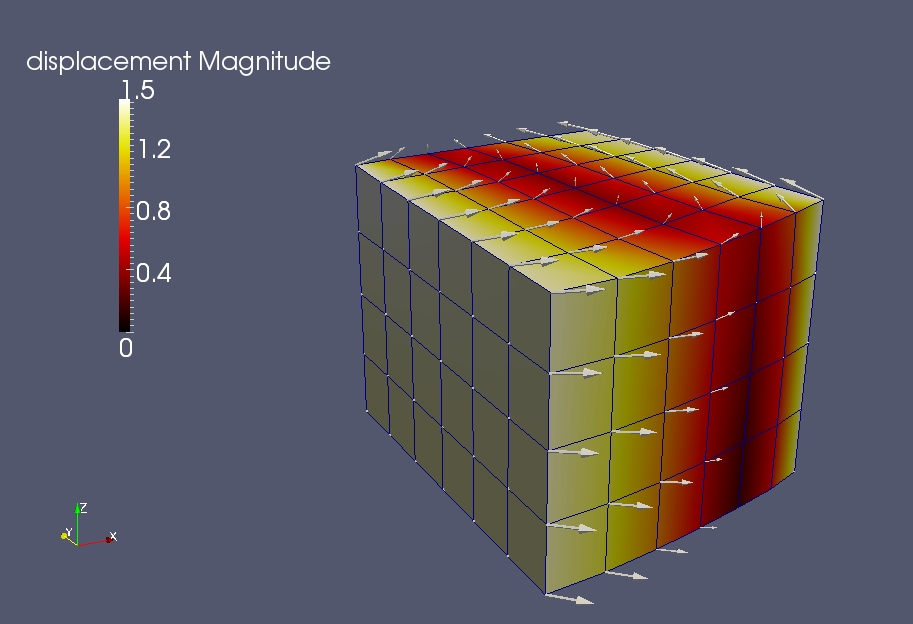
\includegraphics[width=10cm]{examples/figs/3dhex8_step01-displ}
  \caption{Displacement field for example step01 visualized using ParaView. The
    mesh has been distorted by the computed displacements (magnified by
    500), and the vectors show the computed displacements.}
  \label{fig:example:3dhex8:step01:displacement}
\end{figure}


\subsubsection{Step02 - Dirichlet and Neumann Boundary Conditions}

The \filename{step02.cfg} file defines a problem with Dirichlet (displacement)
boundary conditions corresponding to zero x and y-displacements applied
on the negative x-face and Neumann (traction) boundary conditions
corresponding to normal compression and horizontal shear applied on
the positive x-face. The bottom (negative z) boundary is held fixed
in the z-direction. The problem is similar to example step01, except
that 1 MPa of normal compression and 1 MPa of shear (in a left-lateral
sense) are applied on the positive x-face, and the negative x-face
is pinned in both the x and y-directions.

For the boundary conditions, we must first change the boundary condition
type for the positive x-face from the default Dirichlet to Neumann:
\begin{cfg}[Excerpt from \filename{step02.cfg}]
# +x face -- first change bc type to Neumann
<h>[pylithapp.timedependent.bc]</h>
<f>x_pos</f> = pylith.bc.Neumann 
\end{cfg}
We use a \object{SimpleDB} to describe the traction boundary
conditions.  When applying traction boundary conditions over a
surface, it is also necessary to specify integration information for
the surface. Since this is a three-dimensional problem, the dimension
of the surface is 2. Since the cells being used are trilinear
hexahedra, the cell type is \object{FIATLagrange} and we use an
integration order of 2.  A lower integration order would not provide
sufficient accuracy while a higher integration order would offer no
benefit (while requiring more computation time and storage):
\begin{cfg}[Excerpt from \filename{step02.cfg}]
# Boundary condition on +x face
<h>[pylithapp.timedependent.bc.x_pos]</h>
<p>label</p> = face_xpos
<f>db_initial</f> = spatialdata.spatialdb.SimpleDB
<p>db_initial.label</p> = Neumann BC on +x
<p>db_initial.iohandler.filename</p> = spatialdb/tractions_axial_shear.spatialdb

# We must specify quadrature information for the cell faces.
<f>quadrature.cell</f> = pylith.feassemble.FIATLagrange
<p>quadrature.cell.dimension</p> = 2
<p>quadrature.cell.quad_order</p> = 2 
\end{cfg}
The boundary conditions on the negative x-face are simpler than they
were in example step01 (zero displacements in the x and y-directions),
so we can use the default \object{ZeroDispBC}:
\begin{cfg}[Excerpt from \filename{step02.cfg}]
# Boundary condition on -x face
<h>[pylithapp.timedependent.bc.x_neg]</h>
<p>bc_dof</p> = [0, 1] 
<p>label</p> = face_xneg
<p>db_initial.label</p> = Dirichlet BC on -x 
\end{cfg}
The boundary conditions on the negative z-face are supplied in the
same manner as for example step01. When we have run the simulation,
the output VTK files will be contained in \filename{examples/3d/hex8/output}
(all with a prefix of \filename{step02}). Results using ParaView are
shown in Figure \vref{fig:example:3dhex8:step02:displacement}.

\begin{figure}
  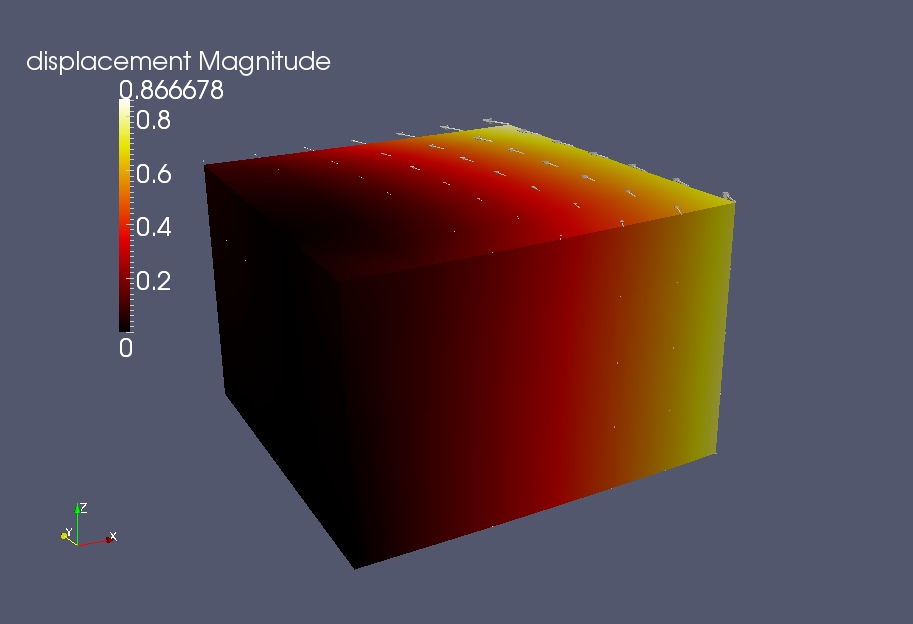
\includegraphics[width=10cm]{examples/figs/3dhex8_step02-displ}
  \caption{Displacement field for example step02 visualized using ParaView. The
    mesh has been distorted by the computed displacements (magnified by
    500), and the vectors show the computed displacements.}
  \label{fig:example:3dhex8:step02:displacement}
\end{figure}


\subsubsection{Step03 - Dirichlet Boundary Conditions with Kinematic Fault Slip}

The \filename{step03.cfg} file describes a problem with Dirichlet (displacement)
boundary conditions corresponding to zero x and y-displacements applied
on the negative and positive x-faces and a vertical fault with a combination
of left-lateral and updip motion. The left-lateral component of fault
slip has a constant value of 2 m in the upper crust, and then decreases
linearly to zero at the base of the model. The reverse slip component
has a value of 0.25 m at the surface, and then decreases linearly
to zero at 2 km depth.

Due to the simplicity of the boundary conditions, we are able to use
the default \object{ZeroDispBC} for the positive and negative x-faces,
as well as the negative z-face. To use a fault, we must first define
a fault interface. We do this by providing an array containing a single
interface. For this example we specify the fault slip, so we set the interface
type to \object{FaultCohesiveKin}.
\begin{cfg}[Excerpt from \filename{step03.cfg}]
<h>[pylithapp.timedependent]</h>
# Set interfaces to an array of 1 fault: 'fault'.
<f>interfaces</f> = [fault] 

# Set the type of fault interface condition.
<h>[pylithapp.timedependent.interfaces]</h>
<f>fault</f> = pylith.faults.FaultCohesiveKin 

<h>[pylithapp.timedependent.interfaces.fault]</h>
# The label corresponds to the name of the nodeset in CUBIT/Trelis.
<p>label</p> = fault

# We must define the quadrature information for fault cells.
# The fault cells are 2D (surface).
<f>quadrature.cell</f> = pylith.feassemble.FIATLagrange
<p>quadrature.cell.dimension</p> = 2 
\end{cfg}
We retain the default \object{StepSlipFn} since we want static fault
slip. Finally, we use one \object{SimpleDB} to define the spatial
variation of fault slip, and another \object{SimpleDB} to define the
spatial variation in slip initiation times (the start time is 0.0
everywhere since this is a static problem):
\begin{cfg}[Excerpt from \filename{step03.cfg}]
# The slip time and final slip are defined in spatial databases.
<h>[pylithapp.timedependent.interfaces.fault.eq\_srcs.rupture.slip\_function]</h>
<p>slip.iohandler.filename</p> = spatialdb/finalslip.spatialdb
<p>slip.query_type</p> = linear
<p>slip_time.iohandler.filename</p> = spatialdb/sliptime.spatialdb 

# Fault output, give the basename for the VTK file.
<h>[pylithapp.problem.interfaces.fault.output]</h>
<p>writer.filename</p> = output/step03-fault.vtk 
\end{cfg}
This will result in two extra files being produced. The first file
(\filename{step03-fault\_info.vtk}) contains information such as the
normal directions to the fault surface, the applied fault slip, and
the fault slip times. The second file
(\filename{step03-fault\_t0000000.vtk}) contains the cumulative fault
slip for the time step and the change in tractions on the fault
surface due to the slip. When we have run the simulation, the output
VTK files will be contained in \filename{examples/3d/hex8/output} (all
with a prefix of \filename{step03}). Results using ParaView are shown
in Figure \vref{fig:example:3dhex8:step03-displacement}.

\begin{figure}
  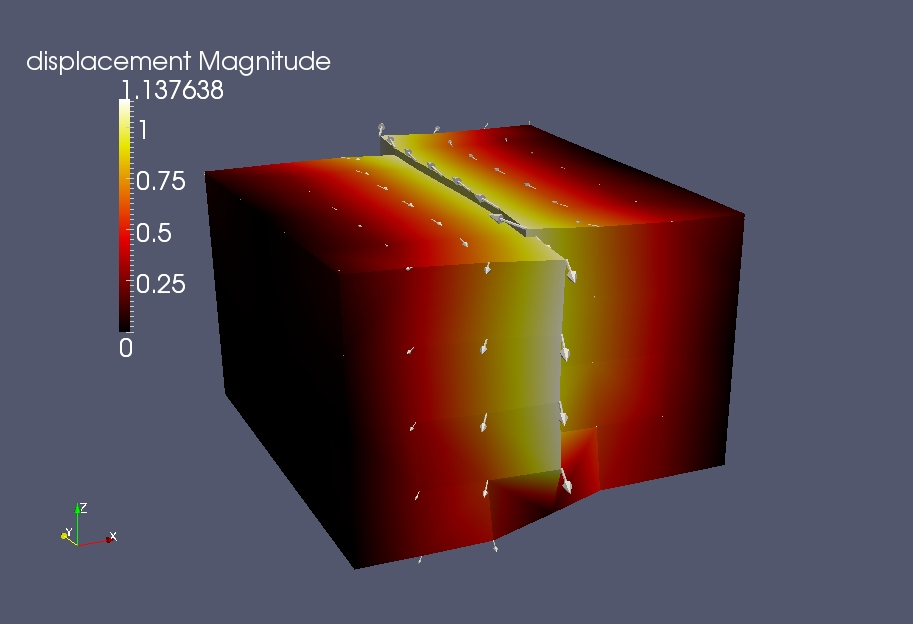
\includegraphics[width=10cm]{examples/figs/3dhex8_step03-displ}
  \caption{Displacement field for example step03 visualized using ParaView. The
    mesh has been distorted by the computed displacements (magnified by
    500), and the vectors show the computed displacements.}
  \label{fig:example:3dhex8:step03-displacement}
\end{figure}


% End of file
